\chapter{Technologies}
\label{chap:Chapter3}
%-------------------------------------------------------------------------------%

\section{Battery Module}

Batteries are a critical component in portable embedded systems, providing the necessary energy for the system to work properly.

This way, the battery technology selection must be carefully made to optimize the system performance, \cite{BATT3}.
Different battery chemistries offer varying energy densities, voltages, sizes, weights, cycle lives and costs.

In table \ref{tab:battery_comparison} it is possible to compare the most common battery technologies.

\begin{table}[H]
    \centering
    \resizebox{\textwidth}{!}{
        \begin{tabular}{lccccc}
            \hline
            \textbf{Technology} & \begin{tabular}[c]{@{}c@{}}\textbf{Energy}\\ \textbf{Density}\end{tabular} & \textbf{Voltage} & \textbf{Size/Weight} & \textbf{Cycle Life} & \textbf{Cost} \\ \hline
            \textbf{Li-ion}     & High                                                                       & 3.7V             & Compact/Light        & Good                & Moderate      \\
            \textbf{Li-Po}      & High                                                                       & 3.7V             & Flexible/Light       & Good                & Moderate      \\
            \textbf{NiMH}       & Moderate                                                                   & 1.2V             & Bulky/Heavy          & Moderate            & Moderate      \\
            \textbf{NiCd}       & Moderate                                                                   & 1.2V             & Bulky/Heavy          & Good                & Moderate      \\
            \textbf{Lead-Acid}  & Low                                                                        & 2V (6V, 12V)     & Bulky/Heavy          & Moderate            & Low           \\
            \textbf{Alkaline}   & Moderate                                                                   & 1.5V             & Standard Cylindrical & Poor                & Moderate      \\
        \end{tabular}%
    }
    \caption{Comparison of Battery Technologies}
    \label{tab:battery_comparison}
\end{table}

\gls{Li-ion} and \gls{Li-Po} batteries, shown in figures \ref{fig:18650} and \ref{fig:lipo}, can offer high energy density, rechargeability and moderate costs that make them suitable for portable devices, \cite{BATT7}.
These batteries stand out as a prevalent choice for embedded systems.
\begin{figure}[H]
    \centering
    \begin{minipage}{.5\textwidth}
        \centering
        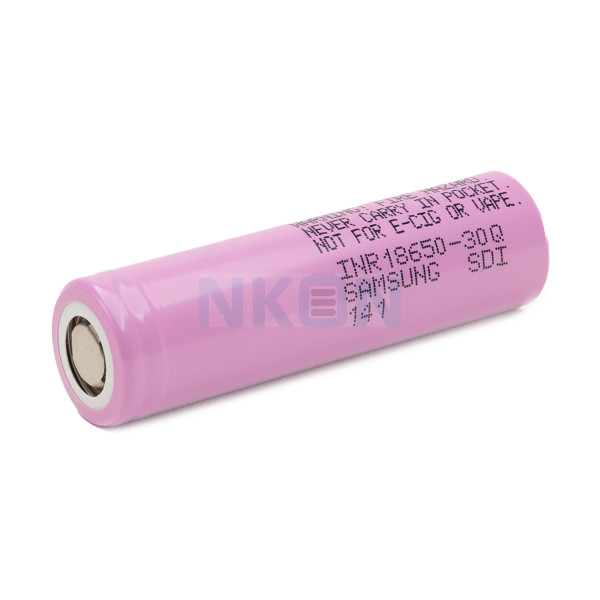
\includegraphics[width=.5\linewidth]{ch3/assets/18650.jpg}
        \captionof{figure}{\gls{Li-ion} battery example \cite{18650}}
        \label{fig:18650}
    \end{minipage}%
    \begin{minipage}{.5\textwidth}
        \centering
        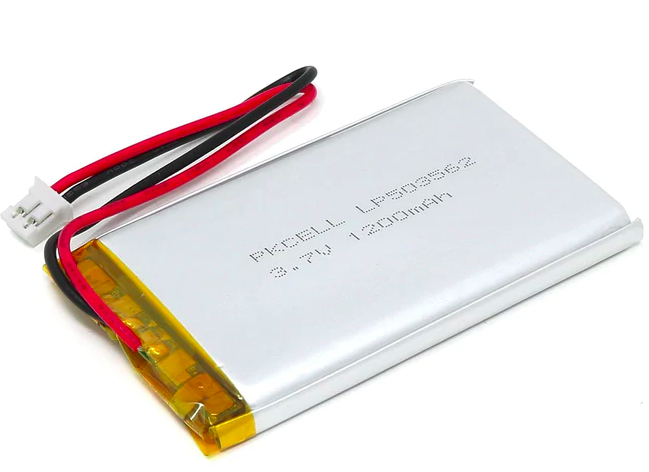
\includegraphics[width=.5\linewidth]{ch3/assets/lipo.png}
        \captionof{figure}{\gls{Li-Po} battery example \cite{lipo}}
        \label{fig:lipo}
    \end{minipage}
\end{figure}

\gls{NiMH} and \gls{NiCd} batteries (figures \ref{fig:nimh} and \ref{fig:nicd} respectably) can provide moderate energy density, rechargeability and moderate costs, but they can be heavier and \gls{NiCd} batteries have a \textit{memory effect} concern (where the battery, falsely, indicates full charge despite being only partially charged).
\begin{figure}[H]
    \centering
    \begin{minipage}{.5\textwidth}
        \centering
        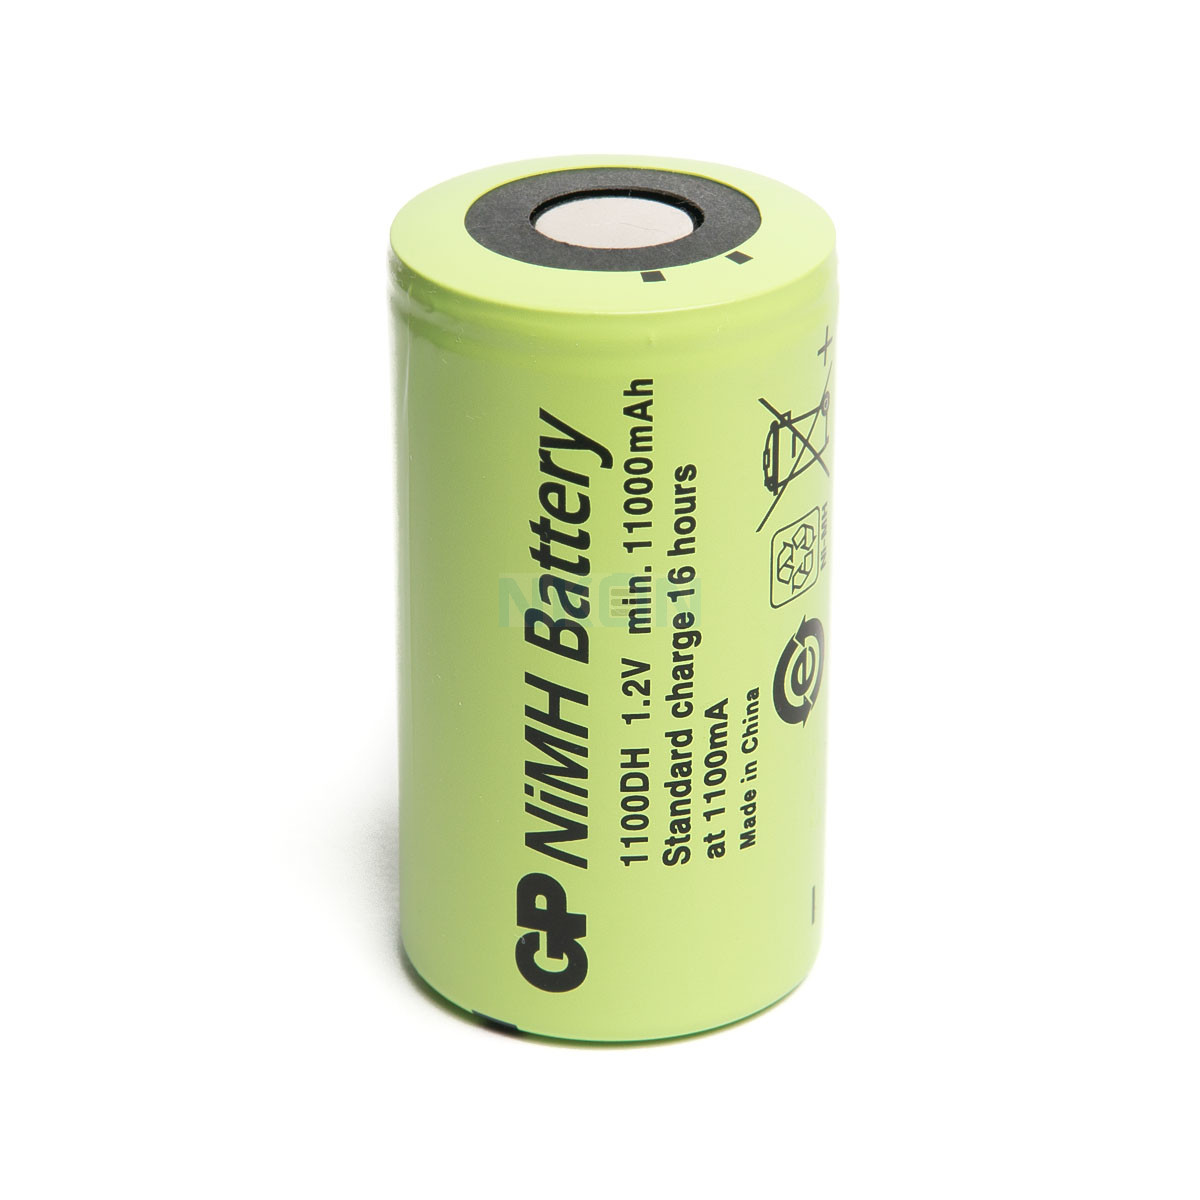
\includegraphics[width=.5\linewidth]{ch3/assets/nimh.jpg}
        \captionof{figure}{\gls{NiMH} battery example \cite{nimh}}
        \label{fig:NiMH}
    \end{minipage}%
    \begin{minipage}{.5\textwidth}
        \centering
        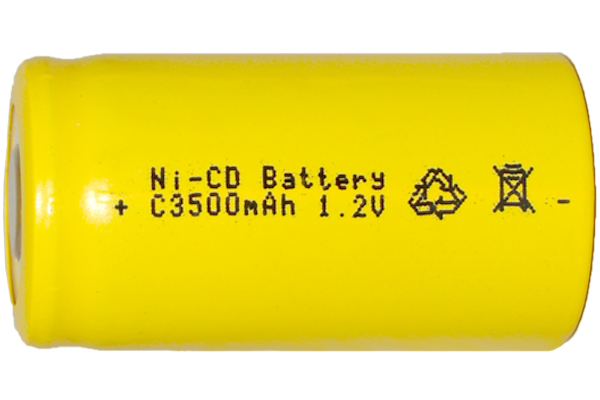
\includegraphics[width=.5\linewidth]{ch3/assets/nicd.jpg}
        \captionof{figure}{\gls{NiCd} battery example \cite{nicd}}
        \label{fig:NiCd}
    \end{minipage}
\end{figure}

Lead-Acid batteries can be rechargeable and cost-effective but heavier and larger and with low energy density.
These batteries are suitable for less portable applications, \cite{BATT3} as it is possible to see in figure \ref{fig:lead}.
\begin{figure}[H]
    \centering
    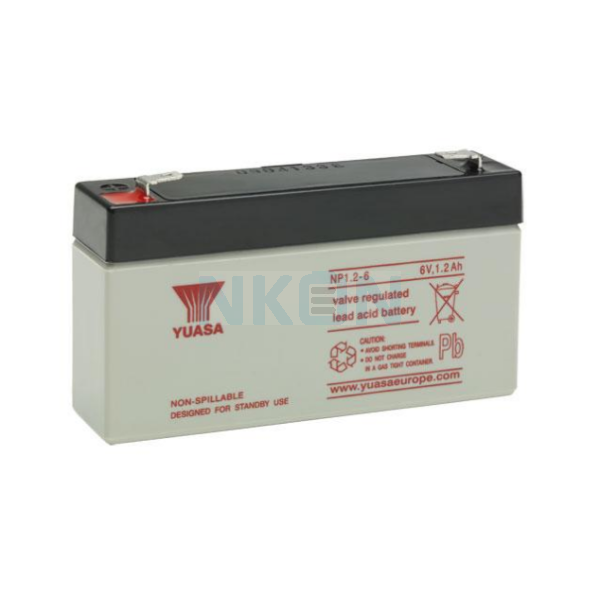
\includegraphics[scale=0.4]{ch3/assets/lead.png}
    \caption{Lead-Acid battery example \cite{lead}}
    \label{fig:lead}
\end{figure}


Alkaline batteries in figure \ref{fig:alkaline} are cost-effective but most of them are non-rechargeable, have a standard cylindrical format and have moderate energy density \cite{BATT3}.
\begin{figure}[H]
    \centering
    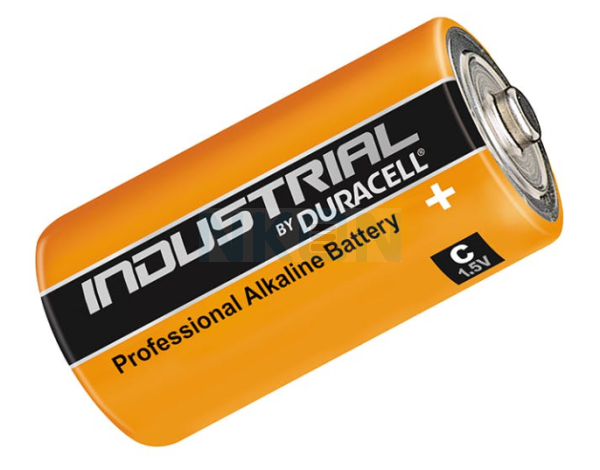
\includegraphics[scale=0.3]{ch3/assets/alkaline.png}
    \caption{Alkaline battery example \cite{alkaline}}
    \label{fig:alkaline}
\end{figure}


%-------------------------------------------------------------------------------%

\section{External Memory and Storage Units}

Memory units can be classified as volatile memory and as non-volatile memory \cite{mem3}.

Volatile storage, like for example \gls{RAM} provides fast read and write speeds and is used for storing variables and managing application stacks.
However, they require constant power to retain data, making them unsuitable for applications with strict power constraints, and have lower memory capacity \cite{mem8}.

Non-volatile storages are suitable for applications requiring frequent data read and write operations and have the capability of being electrically erased and reprogrammed.
They have long-term data retention and low power consumption but have slow access speed compared to volatile storage \cite{mem8}.
These characteristics make non-volatile storages useful for storing configuration parameters and critical data that need to be retained during power cycles.

Often, in embedded systems, the system must be able to store data not only internally (main memory) but also externally (external memory).
External memory units are normally used to expand storage capacity, store data and logs, facilitate data transfer, and backup critical information \cite{mem3}.

Since non-volatile storage can keep the data stored even when they are not powered, these storages are very common in embedded systems \cite{mem1}.

\gls{SD} card, with its multiple formats and sizes, has moderate access speed and can keep data for a long term but it depends on the type (\gls{SLC}, \gls{MLC} and \gls{TLC}).
Typically, the capacity ranges from a few megabytes to multiple terabytes, offering multiple choices for different use cases \cite{mem11}, \cite{mem9}.
However, the moderate power consumption and overall cost can, sometimes, be a setback to the system.

\gls{EEPROM}, commonly used for storing small amounts of data, has fast access speed and a moderate overall cost.
Has long-term data retention and low power consumption but offers lower capacities (in the range of kilobytes to megabytes) making it only suitable for small data storage \cite{mem8}, \cite{mem11}.

\gls{FRAM} combines the benefits of \gls{RAM} and \gls{EEPROM} and can be suitable for applications requiring fast and non-volatile memory.
Has very fast access speed, long-term data retention, low capacity (in the range of kilobytes to megabytes), and very low power consumption.
But has a relatively higher overall cost compared to other technologies \cite{mem8}, \cite{mem11}.

As for \gls{eMMC}, normally found in smartphones, tablets, and other embedded systems, is characterized by its fast access speed, long-term data retention and high capacity (with ranges from megabytes to terabytes).
Like \gls{SD} cards it has moderate power consumption and moderate to high overall cost \cite{mem11}.

\gls{HDD} and \gls{SSD} memory units can have fast access speed, long-term data retention and high capacity (in the range of gigabytes to terabytes).
But, in comparison to other memory units, it has a bigger size, higher power consumption and higher overall cost.
These units are normally used as primary storage in computers and laptops for improved performance, \cite{mem10}.

Table \ref{tab:memory_comparison} compares the described technologies in their access speed, overall cost, data retention, capacity and power consumption.
\begin{table}[H]
    \centering
    \resizebox{\textwidth}{!}{
        \begin{tabular}{lcccccc}
            \hline
                              & \textbf{Access Speed} & \textbf{Overall Cost} & \textbf{Data Retention} & \textbf{Capacity} & \textbf{Power Consumption} \\ \hline
            \textbf{SD Cards} & Moderate              & Moderate              & Long-term               & High              & Moderate                   \\
            \textbf{EEPROM}   & Fast                  & Moderate              & Long-term               & Low               & Low                        \\
            \textbf{FRAM}     & Very Fast             & Relatively Higher     & Long-term               & Low               & Very Low                   \\
            \textbf{eMMC}     & Fast                  & Moderate              & Long-term               & High              & Moderate                   \\
            \textbf{SSD}      & Very Fast             & High                  & Long-term               & Very High         & High                       \\
            \textbf{HDD}      & Moderate              & High                  & Long-term               & very High         & High                       \\\hline
        \end{tabular}
    }\caption{Comparison of External Memory Technologies}
    \label{tab:memory_comparison}
\end{table}

\section{Firmware}
In embedded systems, the choice of programming languages and the use of a \gls{RTOS} in firmware development are critical decisions that can impact the performance, efficiency, and complexity of the embedded system.

\subsection{Programming languages}
Even though there are multiple programming languages, normally categorized as low-level or high-level, not all programming languages are optimized to be used in embedded systems.
In this section, an overview and comparison were made on some examples of programming languages \cite{LPROG4}, \cite{LPROG6}.

\subsubsection{C}
\textit{C} programming language has low-level features and is close to the hardware making it efficient and with high performance \cite{LPROG2}, \cite{LPROG6}.

It provides fine-grained control over memory, leading to efficient memory usage but can also lead to potential errors if not handled carefully \cite{LPROG5}.
Due to its low-level control and predictable performance, it is often used in real-time systems \cite{LPROG7}.

This programming language is generally portable and has a large and active community, with extensive support and numerous libraries, development tools and compilers available \cite{LPROG7}.

In terms of safety and reliability, it is a powerful language but lacks some safety features, like in memory management for example \cite{LPROG7}.

\textit{C} can have a steeper learning curve, especially for beginners, due to manual memory management and low-level constructs \cite{LPROG2}.

\subsubsection{Assembly}
\textit{Assembly} programming language provides direct control over hardware and is highly efficient, and useful for writing low-level code.
It allows developers to directly manage memory, providing fine control over memory footprint \cite{LPROG7}.

\textit{Assembly} can be used in real-time systems due to its precise control over hardware, predictable performance and high efficiency \cite{LPROG5}.

However, in \textit{Assembly}, there is no safety net or restrictions, this way developers must handle all aspects of safety and reliability manually \cite{LPROG7}.
\textit{Assembly} is also highly dependent on the architecture and is not inherently portable, has a niche community, and support is often architecture-specific and relies on specific tools provided by the hardware manufacturer.
The learning curve is steep due to its low-level nature, and development is time-consuming compared to higher-level languages \cite{LPROG5}.

\subsubsection{C++}
\textit{C++} programming language is an object-oriented feature that can enhance code organization and reusability and can provide abstraction without sacrificing performance.
It allows both manual and automatic memory management, providing flexibility \cite{LPROG2}, \cite{LPROG6}.
\textit{C++} supports real-time programming, especially with the use of specific frameworks but is not as deterministic as low-level languages.

This programming language benefits from a robust community, with extensive support, it inherits development tools and compilers from \textit{C} and has specific tools for features like object-oriented programming \cite{LPROG7}.

C++ introduces features like classes and objects, enhancing code organization and safety compared to C.
However, it still allows low-level operations that may impact reliability \cite{LPROG5}.

Since \textit{C++} is similar to \textit{C}, and since it introduces additional concepts, the learning curve can be slightly more complex.
However, its object-oriented features can lead to more maintainable code \cite{LPROG7}.

\subsubsection{Rust}
\textit{Rust} programming language, known for its focus on memory safety, is gaining popularity in embedded systems development.
It offers performance similar to \textit{C} and \textit{C++} while providing memory safety features \cite{LPROG2},\cite{LPROG7} .

\textit{Rust's} was designed with a strong focus on memory safety with an ownership system that helps prevent common memory-related errors without sacrificing performance.
This results in a secure and efficient memory footprint \cite{LPROG2}.

As for portability, it aims to be highly portable, with a focus on minimizing platform-specific issues.
With features like Cargo, it simplifies dependency management and project setup.

\textit{Rust} has a growing community and is gaining popularity, with strong support.
However, it can be challenging for beginners due to its ownership system \cite{LPROG7}.

\subsubsection{MicroPython}
\textit{MicroPython} is a compact extension of Python designed for microcontrollers and IoT devices to emphasize efficiency.
However, it sacrifices some features of the standard Python to fit within resource constraints \cite{LPROG2}.

It aims for a small memory footprint suitable for microcontrollers which enhances portability as well \cite{LPROG7}.

\textit{MicroPython} can be used for real-time tasks on microcontrollers, but its capabilities may be limited since it is not as deterministic as low-level languages.
The community focused on supporting embedded systems for \textit{MicroPython} is growing with resources specifically tailored to microcontroller development \cite{LPROG2}, \cite{LPROG5}.

Table \ref{tab:programming_languages_comparison} resumes and compares all programming languages described above.
\begin{table}[H]
    \centering
    \resizebox{\textwidth}{!}{
        \begin{tabular}{lcccccc}
            \hline
            \textbf{Topic}             & \textbf{C} & \textbf{C++} & \textbf{Rust} & \textbf{Assembly} & \textbf{MicroPython} \\ \hline
            Efficiency and Performance & High       & High         & High          & Very High         & Moderate             \\
            Memory Footprint           & Low        & Moderate     & Moderate      & Very Low          & Low                  \\
            Real-Time Capabilities     & Limited    & Limited      & Developing    & Yes               & Limited              \\
            Portability                & High       & Moderate     & Moderate      & Low               & High                 \\
            Community and Support      & Large      & Large        & Growing       & Limited           & Growing              \\
            Development Tools          & Abundant   & Abundant     & Growing       & Limited           & Limited              \\
            Safety and Reliability     & Moderate   & Moderate     & High          & Low               & Moderate             \\
            Learning and Development   & Moderate   & Moderate     & Moderate      & Difficult         & Easy                 \\ \hline
        \end{tabular}
    }
    \caption{Comparison of Programming Languages in Embedded Systems}
    \label{tab:programming_languages_comparison}
\end{table}

\subsection{Real-time Operating Systems}
\glspl{RTOS} facilitates multitasking, allowing concurrent execution of multiple tasks, can provide task scheduling, priority management, and inter-process communication and is suitable for systems with real-time requirements.
But this can add overhead, especially in terms of memory footprint, and the learning curve is steeper \cite{RTOS1}.\\
The following \gls{RTOS} examples are open-source, well-documented, compact, and designed for resource-constrained systems, and they support various microcontroller architectures \cite{RTOS5}.
They also support microROS, an extension of the \gls{ROS}, designed for microcontrollers and embedded systems that can be resource-constrained.
\subsubsection{FreeRTOS}
\textit{FreeRTOS} is a popular open-source (with MIT license) real-time operating system.

It has a small footprint, making it suitable for resource-constrained embedded systems.
Has a large and active community, which can be beneficial for support and finding solutions \cite{RTOS6}.

As for scheduling policies, it has priority-based, round-robin and rate monotonic schedulers and has semaphore/mutex management \cite{compRTOS}.
It supports I2C, SPI and UART wired protocols and BLE-Stack, TLS, Ethernet and  Wifi network protocols \cite{compRTOS}.
\subsubsection{ChibiOS}

\textit{ChibiOS} is a real-time operating system designed for embedded systems with GPL3/commercial license.
It is designed to be modular, allowing the user to include only the necessary components.
This way it can be used for both small and large systems \cite{chibios}. 

Offers a rich set of features, including support for various architectures and a hardware abstraction layer.

\subsubsection{NuttX}
\cite{nuttx}
\cite{compRTOS}

\textit{NuttX} is a real-time operating system with a focus on standards compliance (POSIX and ANSI).
It uses the Apache 2.0 license, allowing for both open-source and commercial use \cite{nuttx}.

\textit{NuttX} can be scalable, providing a balance between small footprint for resource-constrained devices and support for larger systems.

In terms of scheduling Priority-based 	FIFO Round-Robin Sporadic Server Semaphore /Mutex management
I2C SPI USB CAN Modbus

6LoWPAN Ethernet Wifi RFID

\subsubsection{Zephyr}
\cite{RTOS5}
\cite{zephyr}
\cite{compRTOS}

\textit{Zephyr} is a real-time operating system for resource-constrained devices.
It supports micro-ROS, allowing integration with ROS-based robotic systems.
Micro XRCE-DDS is one of the DDS implementations that can be used with Zephyr.

Licensing: Released under the Apache 2.0 license, allowing for open-source and commercial use.
Footprint: Designed to be scalable and can be configured to match the requirements of the target device.
Community: Has a growing and active community. Supported by the Linux Foundation.

Critical Systems Perspective:

    All of these RTOSs can be used in critical systems, but the choice might depend on specific requirements such as certification standards, safety features, and community support.
    Certification: Consider the certification standards required for critical systems, like DO-178C for avionics or ISO 26262 for automotive.



https://micro.ros.org/docs/concepts/rtos/comparison/

Table \ref{tab:rtos_comparison} \cite{compRTOS}.
\begin{table}[H]
    \centering
    \caption{Comparison of Real-Time Operating Systems}
    \label{tab:rtos_comparison}
    \resizebox{\textwidth}{!}{
        \begin{tabular}{lcccc}
            \hline
            \textbf{Feature}      & \textbf{FreeRTOS} & \textbf{ChibiOS}      & \textbf{NuttX} & \textbf{Zephyr} \\ \hline
            Licensing             & MIT               & Mixed GPL3/Commercial & Apache 2.0     & Apache 2.0      \\
            Memory Footprint      & Small             & Small to Large        & Scalable       & Scalable        \\
            Community and Support & Large             & Active                & Growing        & Active          \\
            Architecture Support  & Wide              & Wide                  & Wide           & Wide            \\
            Certification         & Depends           & Depends               & Depends        & Considered      \\
            POSIX/ANSI Compliance & Limited           & Limited               & Yes            & Limited         \\
            Safety Features       & Basic             & Yes                   & Depends        & Depends         \\ \hline
        \end{tabular}
    }
\end{table}


\subsection{Comparison}
Programming Languages:
Pros:

Portability: Higher-level languages like C or C++ provide better portability across different hardware platforms.
Productivity: High-level languages can increase developer productivity by abstracting hardware details and providing more expressive syntax.
Code Reusability: Modular code and libraries are more easily reusable, saving time and effort in development.

Cons:

Performance Overhead: High-level languages may introduce performance overhead compared to low-level languages like assembly or C, which can be critical in resource-constrained embedded systems.
Memory Usage: Applications written in high-level languages might consume more memory compared to optimized low-level code.
Limited Control: Developers may have less control over low-level hardware details, which could be essential for certain embedded applications.

Real-Time Operating Systems (RTOS):
Pros:

Deterministic Timing: RTOS provides deterministic timing, crucial for systems where timing constraints are critical.
Task Management: Efficient task scheduling and management enable the execution of multiple tasks simultaneously.
Resource Management: RTOS can effectively manage resources, optimizing CPU and memory usage.

Cons:

Complexity: Integrating an RTOS can introduce complexity, especially for small-scale embedded systems where simplicity is essential.
Overhead: Some RTOS overhead is incurred in terms of both processing time and memory usage.
Learning Curve: Developers may need to invest time in learning and understanding the specific RTOS, adding to the development time.





%-------------------------------------------------------------------------------%

\section{Communication}
TODO: MORE INFO\\
\subsection{Wired}
TODO: MORE INFO\\

\subsection{Wireless}
While researching wireless communication, multiple protocols can be studied. They can, mainly, be separated into two categories: short-range and long-range.
In the context of \glspl{uav}, the focus will be on short-range wireless communication protocols \cite{WCOM1}, \cite{WCOM6}, \cite{WCOM7}.

Short-range protocols offer advantages such as lower power consumption, reduced interference, and efficient data transfer within confined spaces.
Within this category, options like Bluetooth, Wi-Fi, Zigbee, Z-Wave, and LoRa for short distances emerge as noteworthy candidates.
Each of these protocols addresses specific requirements, making them suitable for various aspects of \gls{uav} operations, from intra-component communication to data transfer between the \gls{uav} and ground control \cite{WCOM6}, \cite{WCOM7}.

\begin{itemize}
    \item WiFi (802.11x): Can be used for high-speed data transfer over short ranges. It's suitable when you need to transmit large amounts of data between the \gls{uav} and a ground station.
          \begin{itemize}
              \item Advantages
                    \begin{itemize}
                        \item High Data Rates
                        \item Widespread Standard
                        \item Bi-Directional Communication
                    \end{itemize}
              \item Disadvantages
                    \begin{itemize}
                        \item High Power Consumption
                        \item Interference in 2.4 GHz and 5 GHz bands
                    \end{itemize}
          \end{itemize}

    \item Bluetooth: Common short-range wireless technology with low power consumption. It's suitable for communication between components on a \gls{uav}.
    \item Advantages
          \begin{itemize}
              \item Low Power Consumption
              \item Ubiquity
          \end{itemize}
    \item Disadvantages
          \begin{itemize}
              \item Limited Range
              \item Data Transfer Rates
          \end{itemize}

    \item Zigbee: Low-power, low-data-rate wireless communication technology that is suitable for short-range communication in embedded systems.
    \item Advantages
          \begin{itemize}
              \item Low Power Consumption
              \item Mesh Networking
              \item Low Latency
          \end{itemize}
    \item Disadvantages
          \begin{itemize}
              \item Limited Data Rate
              \item Limited Range
          \end{itemize}

    \item Z-Wave: Low-power wireless communication protocol often used in home automation. It's suitable for control and monitoring applications in \glspl{uav}.
    \item Advantages
          \begin{itemize}
              \item Low Power Consumption
              \item Interference Avoidance
          \end{itemize}
    \item Disadvantages
          \begin{itemize}
              \item Limited Data Rate
              \item Less Common in Non-Home Automation Devices
          \end{itemize}

    \item LoRa (Long Range): While designed for long-range communication, LoRa can also be used in short-range applications. It provides low-power, long-range communication suitable for certain \gls{uav} scenarios.
    \item Advantages
          \begin{itemize}
              \item Long Range
              \item Low Power Consumption
          \end{itemize}
    \item Disadvantages
          \begin{itemize}
              \item Low Data Rates
              \item Unidirectional Communication
          \end{itemize}
\end{itemize}

%-------------------------------------------------------------------------------%

% \section{Power Management System}
% TODO: MORE INFO\\

% \subsection{Power Distribution}
% TODO: MORE INFO\\

% \subsection{Battery Protection}
% \gls{UVP}\\
% Fuse (but a single point of failure)\\
% Reverse polarity Protection\\
% TODO: MORE INFO\\

%-------------------------------------------------------------------------------%